\chapter{Konzeption}
\label{chapter:Konzeption}

\section{Konzeption der Anwendung} %Benedikt
\label{section:Konzeption der Anwendung} %Benedikt
<<Benedikt>>

\subsection{Grundidee} %Benedikt
\label{subsection:Grundidee} %Benedikt
<<Benedikt>>

\subsection{Mockup} %Benedikt
\label{subsection:Mockup} %Benedikt
<<Benedikt>>

\section{Konzeption des künstlichen neuronalen Netzes}
\label{section:Konzeption des künstlichen neuronalen Netzes}

in den folgenden Abschnitten wird ein \acs{knn} konzeptioniert, dass als Vorlage für alle zu erstellenden \acs{knn} zur Prognose von Börsenkursen dienen soll. 

\subsection{Wahl des Netztyps}
\label{subsection:Wahl des Netztyps}
Zunächst ist zu ermitteln, welche Netztypen sich zur Prognose von Börsenkursen grundsätzlich eignen. Nicht jeder Netztyp ist gleichermaßen zur Prognose geeignet. Bestimmte \acs{knn} sind sogar überhaupt nicht in der Lage, bestimmte Prognosen zu erstellen. 

Grundsätzlich lassen sich \acs{knn} in zwei Oberklassen unterteilen. Die Hetero-Assoziativen Netze sowie die Auto-Assoziativen Netze. Hetero-Assoziative Netze bilden einen Vektor $A$ der Länge $n$ auf einem Vektor $B$ einer meist kürzeren Länge $m$ $\{m \in \mathbb{N} | m \le n\}$ ab. Auto-Assoziative Netze wiederum bilden einen Eingabevektor der Länge $n$ auf einem Ausgabevektor der gleichen Länge ab. Innerhalb dieser zwei Klassen lassen sich \acs{knn} wiederum in mehrere Netztypen aufteilen. Die folgende Tabelle liefert hierzu eine Übersicht:

\begin{center}
\begin{tabular}{|c|c|}
\hline 
\textbf{Hetero-assoziative Netzmodelle} & \textbf{Auto-assoziative Netzmodelle} \\ 
\hline 
(M)Adaline & Hopfield-Netze \\ 
\hline  
Perzeptron &  Boltzmann Maschinen \\ 
\hline 
Multilayerperzeptron & - \\ 
\hline 
\end{tabular} 
\end{center}

Das \acs{knn} soll mithilfe mehrerer vorhergehender Börsenkurse den zukünftigen Börsenkurs prognostizieren. Da es sich bei dem Börsenkurs um einen skalaren Wert handelt, ist die Anzahl der Eingabeneuronen (und die Anzahl der Elemente des Eingabevektors) höher als die Anzahl der Ausgabeneuronen (und damit die Anzahl der Elemente des Ausgabevektors). Somit sind für diese Seminararbeit nur Hetero-assoziative Netze von Relevanz.

Aus den Hetero-Assoziativen Netzen ist nun der Netztyp zu ermitteln, der für die Anwendung am geeignetsten ist. D

Zur Wahl eines geeigneten Netztyps kann zunächst die Lineare Separierbarkeit betrachtet werden:

\newmdtheoremenv{defi}{Definition}
\begin{defi}
Seien $X_{0}$ and $X_{1}$ zwei Datenmengen im $n$-dimensionalen euklidischen Raum. Dann sind die Mengen $X_{0}$ and $X_{1}$ genau dann  "`linear separierbar"', wenn es  $n+1$ Werte $w_{1}, w_{2},..,w_{n}, k$, gibt, sodass jeder Punkt  $x \in X_{0}$ die Bedingung $\sum^{n}_{i=1} w_{i}x_{i} > k$ erfüllt und jeder Punkt $x \in X_{1}$ die Bedingung $\sum^{n}_{i=1} w_{i}x_{i} < k$ erfüllt.
\end{defi}

Um das Verständnis der oben genannten Definition zu erleichtern, kann die folgende Abbildung betrachtet werden:

\begin{figure}[H]
\centering
		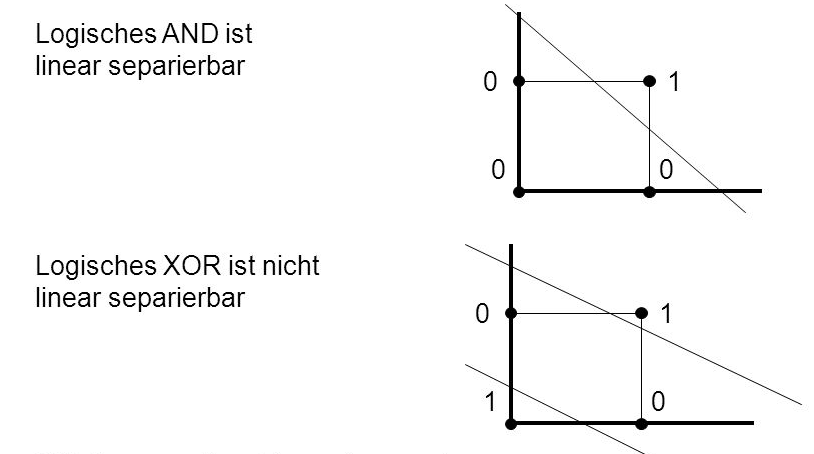
\includegraphics[width=0.95\textwidth]{Linear_Sep.PNG}
	\caption{Grundlegendes Konzept des KNN}
	\label{fig:Grundlegendes Konzept des KNN}
\end{figure}

Man erkennt also, das eine zweidimensionale Funktion dann als linear separierbar gilt, wenn zwischen zwei Ergebnismengen der Funktion eine Gerade gelegt werden kann. Analog setzt sich dies in Funktionen höherer Dimensionen fort. Ist die Funktion zum Beispiel dreidimensional, erfolgt die Separierung erfolgt durch eine Ebene.

Es ist bewiesen, dass einschichtige \acs{knn} nur in der Lage sind, linear separierbare Funktionen zu berechnen.Den Konkreten Beweis dazu liefern dazu Minski \& Papert am Beispiel des XOR-Problems:

\newmdtheoremenv{bew}{Beweis}
\begin{bew}
Gegeben:
das folgende Perzeptron:

\begin{figure}[H]
\centering
		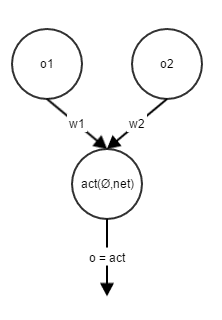
\includegraphics[width=0.15\textwidth]{Perzeptron.PNG}
	\caption{Grundlegendes Konzept des KNN}
	\label{fig:Grundlegendes Konzept des KNN}
\end{figure}

und
$w_1\cdot1 + w_2\cdot2 = net$\\ 
$f_act(o) = id$ \\
$\emptyset = Schwellenwert$\\\

$a) w_1\cdot0 + w_2\cdot0 \le \emptyset$\\
$b) w_1\cdot0 + w_2\cdot0 \geq \emptyset$\\
$c) w_1\cdot0 + w_2\cdot0 \geq \emptyset$\\
$d) w_1\cdot0 + w_2\cdot0 \le \emptyset$\\
 
Widerspruch: $(b+c):  w_1 + w_2 \geq \emptyset  \wedge (d)  w_1 + w_2 \leq \emptyset$ 
 
\end{bew}

\newmdtheoremenv{theo}{Theorem}
\begin{theo}
Konvergenz –Theorem:
   „Der Lernalgorithmus des Perzeptrons konvergiert in endlicher Zeit, d.h. das Perzeptron kann in endlicher Zeit alles lernen, was es repräsentieren                          
   kann.“
\end{theo}

 Perzeptron und die Adaline aber nur linear separierbare Funktionen approximieren können, fallen diese Möglichkeiten weg. Nicht jedoch das mehrschichtige vorwärtsgerichtete Netz. Das dieses \ac{knn} auch tatsächlich dafür geeignet ist, belegt das folgende Theorem:



\begin{theo}
Für ${n \in \mathbb{N} | n>2}$ lässt sich jede reellwertige Funktion $f:[0;1]^n\rightarrow[0;1]$ durch ein dreischichtiges vorwärtsverknüpftes Netz mit maximal $n$ Einheiten in der Eingabeschicht,$(2n+1)$ Einheiten in der Zwischenschicht und $2n+1$ Einheiten in der Ausgabeschicht berechnen.
\end{theo}

Ein Börsenkurs kann prinzipiell jede beliebige Funktion annehmen. Durch das obige Theorem ist jedoch sichergestellt, dass das mehrschichtige vorwärtsgerichtete Netz in der Lage ist, diese Funktionen zu approximieren.


\subsection{Wahl der Topologie}
\label{subsection:Wahl der Topologie}

Zur Prognose werden die vier vergangegen Daten zur Prognose des zukünftigen Wertes als Input Layer genutzt. Da das Ergebnis ein skalarer Wert ist, wir nur ein neurona als Output Layer benötigt. Die optimale Größe des Hidden Layers wird in Punkt (Kapitelverweis) ermittelt. Somit sieht die Topoligie des knn bis jetzt wie golfr aus:

\begin{figure}
\centering
		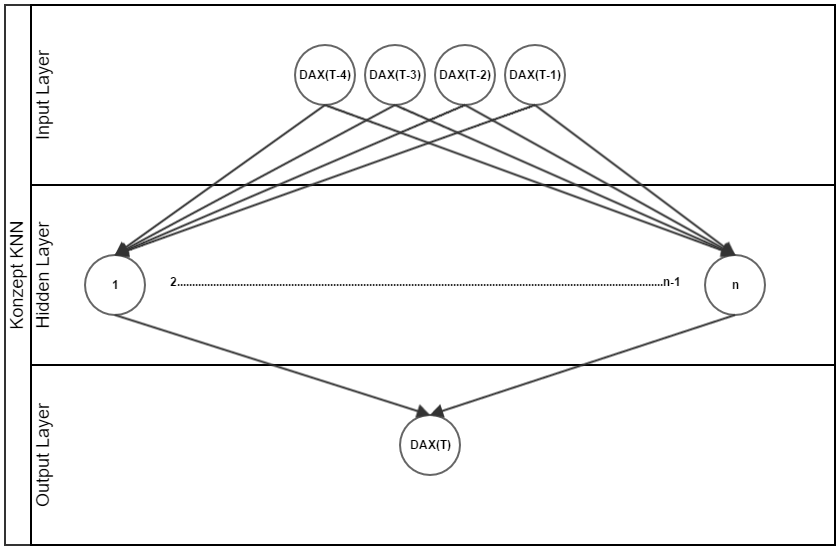
\includegraphics[width=0.95\textwidth]{KonzeptKNN.PNG}
	\caption{Grundlegendes Konzept des KNN}
	\label{fig:Grundlegendes Konzept des KNN}
\end{figure}

\subsection{Wahl des Lernverfahrens} 
\label{subsection:Wahl des Lernverfahrens} 

\subsection{Wahl der Lernrate} 
\label{subsection:Wahl der Lernrate}

